\section{Determine the strength of a poker hand}
\label{sec:part1}
Our first step towards developing an adaptive poker bot is to find a way to determine the strength of any given hand in any game state. In this section we will answer the following problem statement: 

\vspace{4mm}
\begin{statementBox2}{Problem statement 1}
How can one determine the strength of a poker hand?
\end{statementBox2}
\vspace{4mm}

The strength of a hand reflects the probability of winning so the stronger a hand is the more likely one are to win. Since the player does not know the outcome of the community cards during a round of poker, the player has to calculate the probability of winning based on the possible outcomes of the community cards. It is too time consuming to check every outcome as there are more than 250 millions different outcomes of community cards alone. In order to find the probability of winning without having to check all possible outcomes, one can instead make an estimate rather than calculating the true probability. 

\subsection{Design}
When trying to estimate the strength of a hand, two options exist.

The first option is to create a simplified formula. Such formulas already exist, but since they are very simple they tend to be rather inaccurate. This option is straight forward, but the disadvantage is, that it is hard to make a formula that is accurate for every game state.

The second option is to use the Monte Carlo method to simulate a large amount of games and get the distribution of outcomes. This distribution can then be used to find the probability for any of the outcomes.

For a human player a simplified formula is necessary but due to the computational power of a computer the Monte Carlo method is optimal for the APC. The computer can perform thousands of simulations in no time. This method also gives a trade-off between accuracy and the number of simulations. This allows one to adjust the accuracy of the probability by adjusting the number of simulations. The major poker sites also use the Monte Carlo method to determine each players probability of winning.

The solution is implemented as a subsystem that uses the Monte Carlo method. We will refer to this subsystem as the calculator.

\RestyleAlgo{boxruled}
\LinesNumbered
\vspace{4mm}
\begin{algorithm}[H]
  \KwData{Hole cards, number of opponents, community cards (optional)}
  \KwResult{win = 1, draw = 0, lose = -1}
Random missing community cards\;
Determine rank of players hand\;
  \ForEach{opponent} {
    Determine rank of opponents hand\;
    \If{opponent has stronger hand}{\Return ~-1\;}
    \ElseIf{opponent has same hand}{\Return 0\;}
  }
  \Return 1\;
\caption{Pseudo-code for a single simulation}
\end{algorithm}
\vspace{4mm}

The calculator takes three arguments: the hole cards of the player, the number of opponents, and the community cards (optional). The calculator simulates a pre-defined number of rounds and returns an object containing the distribution of wins, draws, and loses.

The calculator considers it a win only if the hand beats every other hand of the opponents.

In order to ensure the quality of the calculator, we have the following requirements:
\begin{itemize}
\item It must be able to return the probability of winning with a given hand in any game state with up to ten players.
\item It must have a maximum error percentage of one percent. (deviation from the true probability)
\item It must calculate the probability in less than three seconds.
\end{itemize}

For requirement one we chose ten players because ten is the maximum number of players in a single round.
For requirement two we chose an error percentage of one because we found it adequate.
For requirement three we chose three second as it seemed fast enough since most players usually have 20-30 seconds for each decision making.

\subsubsection{Monte Carlo method}
The Monte Carlo method is used to find the distribution of outcomes for a domain. Given a set of user defined inputs the Monte Carlo method performs the simulation to find the outcome. For each simulation the method tracks the outcomes and as the number of simulations increases, so will the accuracy of the distribution. This distribution can help to get a better understanding of the domain.

\subsection{Test}
As mentioned earlier the number of simulations affects the accuracy of the result. First we test what number of simulations is needed to fulfil the requirements. 
In order to find the accuracy of the probabilities we first need to know the true probabilities. For this we use caniwin \ref{caniwin}. Caniwin is a website that has simulated all possible outcomes of any pre-flop hands. Caniwin's results are limited to the pre-flop game state, so we can only test the calculator for this game state.\\

After we find an optimal number of simulations we will test the accuracy of the calculator in different game states using this number of simulations.

\subsubsection{Number of simulations}
To find the optimal number of simulations for the calculator we test 
a single hand with a different number of simulations. The calculator calculates the probability 50 times for each test. Each test is performed with the hand J\clubsuit ~ J\diamondsuit ~ in pre-flop with one opponent and the true probability of this is 77,1~\%. We then find the absolute max error and the average computation time of all calculations. The error percentage in table \ref{tab:pre-flop-test} is found using the formula: 

\[err = P_{O} - P_{T}\]

Here $P_{O}$ is the probability found by the calculator and $P_{T} $ is the true probability. 

We plotted the results of each test in a graph, see figure \ref{fig:mc1}, \ref{fig:mc10}, and \ref{fig:mc50}. 
Each test result is indicated with a red dot. The three graphs clearly shows that when using a higher amount of simulations, the more accurate the probability becomes.

The error percentage can be seen in table \ref{tab:mc-total}.


\begin{figure}[H]
  \center
    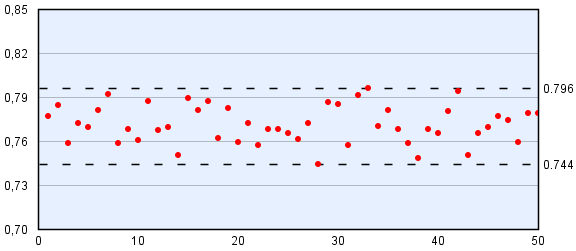
\includegraphics[scale=0.775]{images/MonteCarlo/1k.png}
  \caption{Result of the calculator with 1000 simulations \label{fig:mc1}}
\end{figure}

\begin{figure}[H]
  \center
    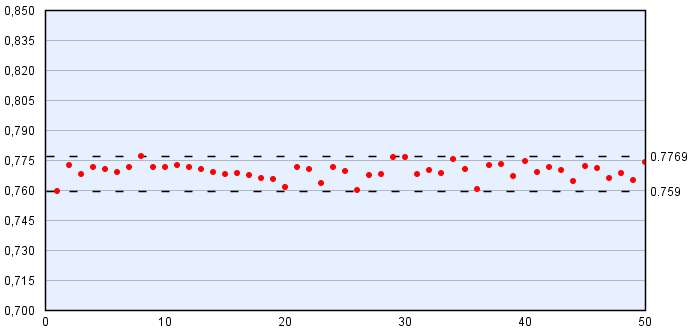
\includegraphics[scale=0.775]{images/MonteCarlo/10k.png}
  \caption{Result of the calculator with 10.000 simulations \label{fig:mc10}}
\end{figure}

\begin{figure}[H]
  \center
    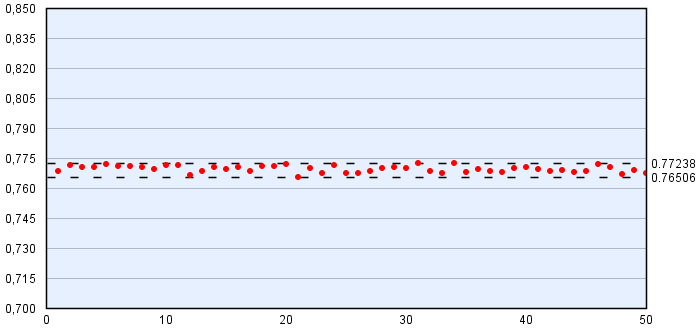
\includegraphics[scale=0.775]{images/MonteCarlo/50k.png}
  \caption{Result of the calculator with 50.000 simulations \label{fig:mc50}}
\end{figure}

We settled for 50.000 as the number of simulations for our calculator. This satisfies our requirements.

\subsubsection{Accuracy of the calculator}
To test if the calculator can calculate the correct probabilities we find the probability of a number of different pre-flop scenarios and compare the result with the results by caniwin. Every test have been preformed with 50.000 simulations against one opponent. The result can be seen in table \ref{tab:pre-flop-test}. From the results we can see that for all hole cards the error percentage is less than one.
\vspace{4mm}
\def\arraystretch{1.5}
\begin{table}[H]
  \center
  \begin{tabular}{ | l | l | l | l | }
  	\hline
  	hole cards & $P_{O}$ (\%) & $P_{T}$ (\%) & error (\%) \\
  	\hline                       
    A\clubsuit ~ A\diamondsuit & 85,2 & 84,9 & 0,3 \\
    8\clubsuit ~ 8\diamondsuit & 67,9 & 68,7 & 0,8 \\
    Q\clubsuit ~ k\clubsuit & 62,8 & 62,4 & 0,4 \\
    A\heartsuit ~ 8\spadesuit & 58,8 & 60,5 & 0,7 \\
    J\spadesuit ~ Q\diamondsuit & 57,2 & 56,9 & 0,3 \\
    10\heartsuit ~ J\heartsuit & 56,7 & 56,2 & 0,5 \\
    3\diamondsuit ~ 3\spadesuit & 53,0 & 52,8 & 0,2 \\
    2\diamondsuit ~ 2\heartsuit & 49,5 & 49,4 & 0,1 \\
    9\diamondsuit ~ 3\spadesuit & 37,8 & 37,4 & 0,4 \\
    2\diamondsuit ~ 7\diamondsuit & 35,5 & 35,4 & 0,1 \\
    2\diamondsuit ~ 7\heartsuit & 31,9 & 31,7 & 0,2 \\
  	\hline   	
  \end{tabular}
  \caption{Test results for different hole cards in pre-flop with one opponent. \label{tab:pre-flop-test}}
\end{table}
\vspace{4mm} 

The pair of fives in table \ref{tab:percent} have a zero percent chance of winning at the river, because the monte carlo does not count a draw as a win.
\vspace{4mm}
\def\arraystretch{1.5}
\begin{table}[H]
  \center
  \begin{tabular}{ | l | l | l | l | l | l | }
  	\hline
  	hole cards & community cards & pre-flop (\%) & flop (\%) & turn (\%) & river (\%) \\
  	\hline 
  	A\clubsuit ~ K\diamondsuit & 3\spadesuit ~ 7\clubsuit ~ T\clubsuit ~ 8\diamondsuit ~ 2\spadesuit & 64,5 & 54,4 & 41,7 & 35,6\\
  	\hline                     
    2\diamondsuit ~ 5\spadesuit & 3\spadesuit ~ 6\diamondsuit ~ K\diamondsuit ~ 4\heartsuit ~ 7\spadesuit & 29,7 & 28,2 & 92,8 & 94,2 \\
    \hline
    8\spadesuit ~ 9\spadesuit & 2\diamondsuit ~ K\spadesuit ~ 3\spadesuit ~ A\clubsuit ~ T\spadesuit & 49,1 & 53,5 & 38,5 & 99,7 \\    
    \hline
    5\spadesuit ~ 5\clubsuit & A\diamondsuit ~ K\heartsuit ~ Q\spadesuit ~ J\diamondsuit ~ T\heartsuit & 58,5 & 48,0 & 34,4 & 0,0 \\    
  	\hline   	
  \end{tabular}
    \caption{Test results for different hole cards in pre-flop, flop, turn, and river with one opponent \label{tab:percent}}
\end{table}
\vspace{4mm} 

Despite a pair of aces is a good hand, the number of opponents makes the chances of winning a lot less
\vspace{4mm}
\def\arraystretch{1.5}
\begin{table}[H]
  \center
  \begin{tabular}{ | l | l | l | l | l | l | l | l | l | l |}
  	\hline
  	opponents & 1 & 2 & 3 & 4 & 5 & 6 & 7 & 8 & 9 \\
  	\hline 
  	win probability (\%) & 85,2 & 73,4 & 64,0 & 56,1 & 49,5 & 43,9 & 39,1 & 35,0 & 31,6 \\
  	\hline                       	
  \end{tabular}
    \caption{Chance of winning with the hole cards A\spadesuit ~ A\clubsuit ~ in pre-flop \label{tab:winchance}}
\end{table}

In table \ref{tab:mc-total} you can see the combined result. The range is the difference between the lowest and highest result and the max error is the maximum deviation from caniwin.

The time have been calculated by finding an average of 100 calculations of the same hole cards.
\vspace{4mm}
\begin{table}[H]
  \center
  \begin{tabular}{ | l | l | l | l | }
    \hline
    simulations & range (\%) & max error (\%) & time (seconds) \\
    \hline                       
    1000 & 5,2 & 2,7 & \textasciitilde{ 0,01} \\
    10.000 & 2,2 & 1,5 & \textasciitilde{ 0.04}\\
    50.000 & 0,9 & 0,7 & \textasciitilde{ 0.15}\\
  \hline  
  \end{tabular}
  \caption{Combined test results from running the calculator with different numbers of simulations. \label{tab:mc-total}}
\end{table}
\vspace{4mm}

\subsection{Discussion}
For the implementation of the calculator the Monte Carlo method was. This method works well for the needs. The calculator can calculate the probability with an error percentage of less than one percent when using 50.000 simulations. This solution can be used for any poker state with up to ten players. At first it did not seem necessary to optimise the calculator any further, as the running time is acceptable. But in regards to later use or if were to scale the project, we decided to make an obvious optimisation by making it multi-threaded which speeded up the calculations by roughly 3 times.	

Since we compare the results of the calculator to caniwin, one would have to ensure the reliability of that source. It is not directly shown who have written the article but when trying to contact the owner of the write we are directed to Bobby. It is very difficult to know if Bobby is the author and whether or not he has any reputation and expertise in the field. However after finding out that the probability from caniwin heads-up and 10 players is very close to the results from the calculator we concluded that caniwin were a reliable source of information.

Alternatively we could have created our own formula to calculate a rank, or used an existing one, for instance the Chen formula. By using this method we will get a less accurate result but it will be easier to calculate. We would also have to create a formula for each game state which would cause even more work. Since performance is not a problem for our calculator we chose to use the Monte Carlo method.

\subsection{Conclusion}
In this section we have answered the question:
\vspace{4mm}
\begin{statementBox2}{Problem statement 1}
How can we predict the probability of ending up with the winning hand?
\end{statementBox2}
\vspace{4mm}

We have implemented a subsystem called the calculator that can estimate the probability of winning with a set of hole cards. The calculator uses the Monte Carlo method and it works for every poker state with up to ten players. We have found that 50.000 simulations is a good number of simulations for our calculator. 

We compare our results to caniwin, which is a website that calculates the actual probabilities of all the 169 combinations of hole cards. The calculator has a maximal error percentage of one percent and performs the simulation in less than a second.
